

\section{Sensori}


\begin{figure}[!ht]
\centering

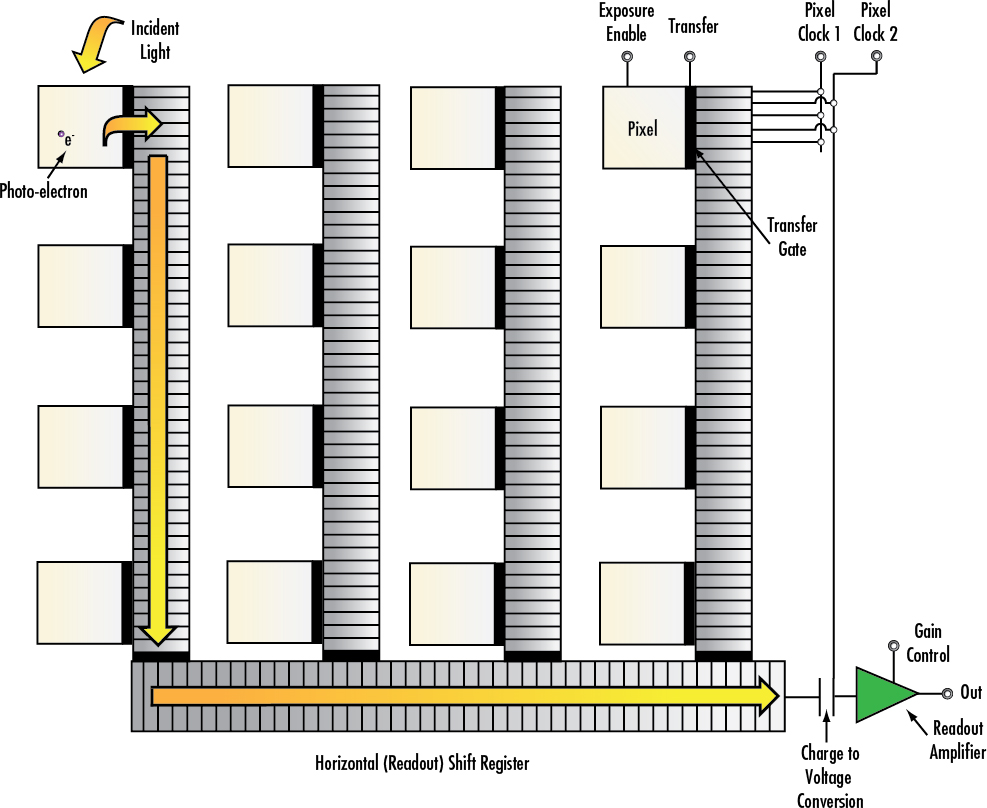
\includegraphics[width=\textwidth]{img/ccd-blockdiagram.jpeg}

\caption{Schema a blocchi di un dispositivo CCD}
\label{fig:ccd-blockdiagram}
\end{figure}

Il cuore di ogni sistema di imaging è il sensore;i moderni sensori sono
dispositivi elettronici a stato solido contenenti fino a milioni di siti
fotorivelatori discreti chiamati pixel.Due telecamere con lo stesso sensore
possono avere prestazioni e proprietà molto differenti a causa della
progettazione dell'elettronica di interfaccia. In passato, le telecamere
utilizzavano fototubi come vidicon e Plumbicons come sensori di immagine.
Anche se non sono più utilizzati, il loro segno sulla nomenclatura associata a
dimensioni del sensore e il formato rimane a questo giorno. Oggi, quasi tutti
i sensori rientrano in una delle due categorie: Charge- Coupled Device (CCD) e
Complementary Metal Oxide Semiconductor (CMOS).

\subsection{CCD} 
Il dispositivo ad accoppiamento di carica (CCD) è stato
inventato nel 1969 da scienziati dei Bell Labs nel New Jersey, Stati Uniti
d'America. Per anni, è stata la tecnologia prevalente per l'acquisizione di
immagini, da astrofotografia digitale a controllo e visione artificiale. Il
sensore CCD è un chip di silicio che contiene una matrice di siti
fotosensibili. Il nome di tale tecnologia si riferisce al metodo con cui i
quanti di carica sono spostati sul chip dai siti fotosensibili fino ad un
registro a scorrimento, simile alla nozione di bucket-brigade (le cariche
vengono passate di ``secchio in secchio''). Impulsi di clock creano buche di
potenziale per spostare quanti di carica sul chip, prima di essere convertito
in una tensione da un condensatore. Il sensore CCD è di per sé un dispositivo
analogico, ma l'uscita viene immediatamente convertita in un segnale digitale
mediante un convertitore analogico-digitale (ADC) on-chip on oppure off-chip.
Nelle fotocamere analogiche, la tensione da ogni sito viene letto in una
particolare sequenza, con impulsi di sincronizzazione aggiunti ad un certo
punto della catena di segnale per la ricostruzione dell'immagine.

La velocità di acquisizione di questa categoria di sensori è limitata dalla
frequenza di trasferimento delle cariche, ciò è però bilanciato da un elevata
sensibilità e consistenza pixel-per-pixel del CCD. Dal momento che ogni quanto
di cariche subisce la stessa conversione di tensione, la resa del CCD è molto
uniforme lungo tutti i suoi siti fotosensibili. Il trasferimento di carica
porta anche al fenomeno della ``blooming'', in cui carica da un sito
fotosensibile si riversa ai siti vicini poichè i singoli elementi hanno una
capacità finita di carica, ponendo un limite superiore della gamma dinamica
utile del sensore. Questo fenomeno si manifesta come macchie di punti
luminosi.

Per compensare la limitata capacità di carica, microlenti sono utilizzate per
aumentare il fattore di riempimento, o la superficie fotosensibile efficace,
per compensare lo spazio sul chip occupata da registri a scorrimento ad
accoppiamento di carica. Questo migliora l'efficienza dei pixel, ma aumenta la
sensibilità angolare di raggi di luce in entrata, richiedendo che colpiscono
il sensore con incidenza normale per la raccolta efficiente.



\begin{figure}[!ht]
\centering

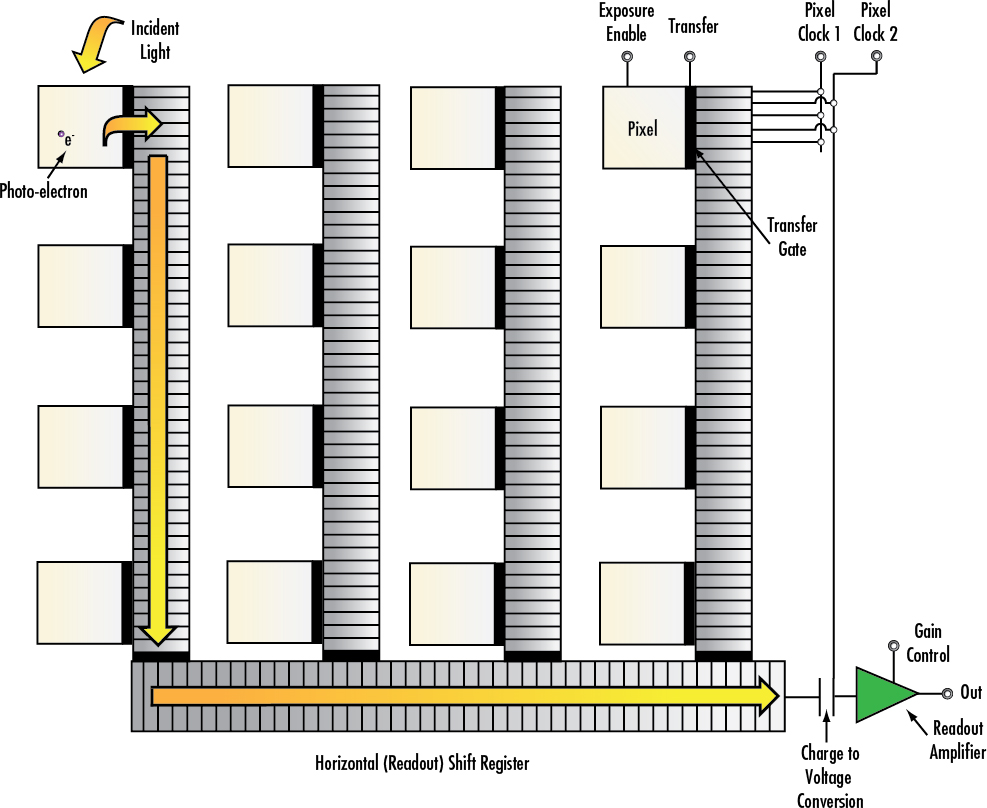
\includegraphics[width=\textwidth]{img/ccd-blockdiagram.jpeg}

\caption{Schema a blocchi di un dispositivo CCD}
\label{fig:ccd-blockdiagram}
\end{figure}

\subsection{CMOS}


Il Complementary metal-oxide semiconductor (CMOS) è stato inventato nel 1963
da Frank Wanlass. Tuttavia, egli non ha ricevuto un brevetto per esso fino al
1967, e non è diventato ampiamente utilizzato per applicazioni di imaging fino
agli anni 1990. In un sensore CMOS, la carica dal pixel fotosensibile viene
convertita in una tensione direttamente sul pixel, il segnale viene
multiplexato per riga e colonna multipla sui chip convertitori digitale-
analogico (DAC). Inerentemente al suo design, il sensore CMOS è un dispositivo
digitale. Ogni sito è essenzialmente un fotodiodo e tre transistori che
svolgono le funzioni di reset o attivazione del pixel, amplificazione e
conversione di carica,  selezione o multiplexing (Figura 2). Questo porta
all'elevata velocità dei sensori CMOS, ma anche una bassa sensibilità e alto
rumore a schema fisso a causa di incongruenze di fabbricazione nei sistemi
multipli di conversione di carica e digitalizzazione.
\begin{figure}[!ht]
\centering

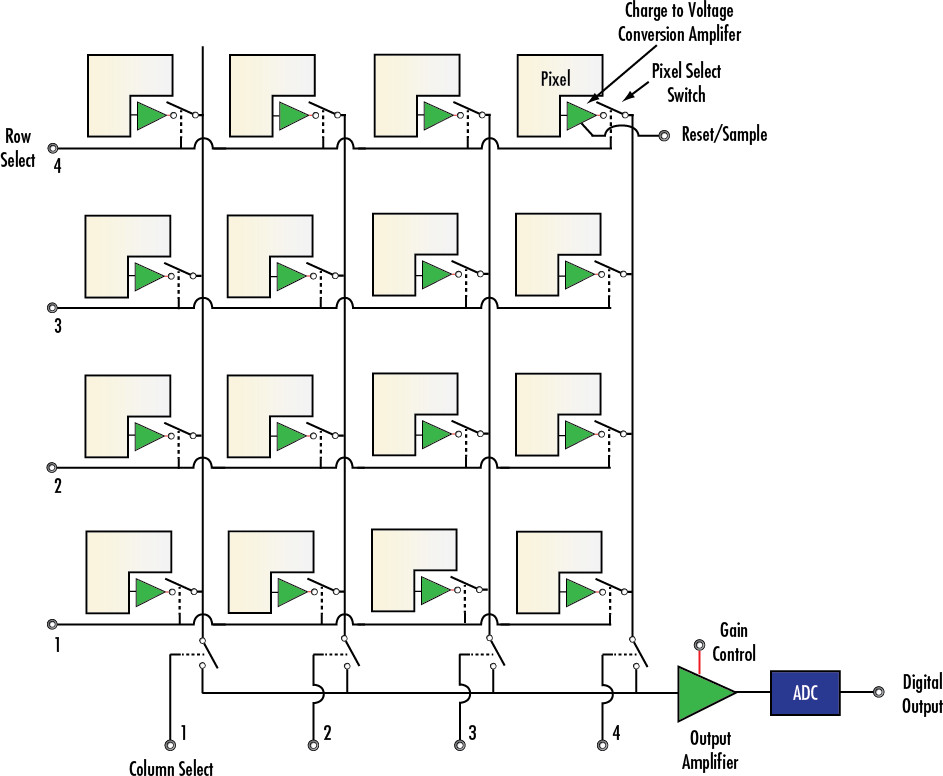
\includegraphics[width=\textwidth]{img/cmos-blockdiagram.jpeg}

\caption{Schema a blocchi di un dispositivo CMOS}
\label{fig:ccd-blockdiagram}
\end{figure}

Un sensore CMOS è spesso accompagnato da un otturatore a scorrimento
elettronico (rolling shutter); sebbene, con ulteriori transistori nel sito del
pixel, un otturatore globale può essere realizzato in cui tutti i pixel sono
esposti simultaneamente per poi procedere ad una lettura sequenziale.

Un ulteriore vantaggio di un sensore CMOS è il suo basso consumo energetico e
dissipazione rispetto ad un sensore CCD equivalente, a causa del minor flusso
di carica, o corrente. Inoltre, la capacità del sensore CMOS di gestire alti
livelli di luce senza blooming permette il suo utilizzo in speciali telecamere
ad alta gamma dinamica.

Il processo di fabbricazione di un sensore CMOS non consente l'uso di
microlenti sul chip, riducendo così l'efficienza di raccolta  del sensore
rispetto ad un equivalente CCD. Questa bassa efficienza combinata con
incongruenza di pixel-per-pixel contribuisce ad un più basso rapporto segnale-
rumore e bassa qualità dell'immagine rispetto ai sensori CCD.

\subsection{Caratteristiche di un sensore}

\subsubsection{Pixel}
Quando la luce colpisce un sensore di imaging essa viene raccolta da una matrice di piccole buche di potenziale chiamati pixel.
 L'immagine è quindi composta elementi discreti. L'informazione viene raccolta da questi siti foto sensibili organizzata, e trasferita.
I pixel possono essere costituiti da fotodiodi o fotocapacitori, per esempio, che generano una carica proporzionale alla quantità di luce incidente su quel luogo discreta del sensore, spazialmente limitato. La capacità di un pixel di convertire un fotone incidente è specificato dalla sua efficienza quantica. Ad esempio, se per dieci fotoni incidenti, quattro foto-elettroni vengono prodotti, allora l'efficienza quantica è del 40\%. Tipici valori di efficienza quantica per imager a stato solido sono nella gamma del 30\% - al 60\%. L'efficienza quantica dipende dalla lunghezza d'onda e non è necessariamente uniforme. Curve di risposta spettrale spesso specificano l'efficienza quantica in funzione della lunghezza d'onda.
Nelle fotocamere digitali, i pixel sono in genere quadrati. Dimensioni dei pixel comuni sono tra 3 - 10 \unit{$\mu m$}. Sebbene per i sensori è spesso indicato semplicemente il numero di pixel, la dimensione è molto importante per l'imaging. Grandi pixel sono, in, grado di arrivare a saturazione con cariche più alte e di avere un rapporto segnare rumore migliore. Con piccoli pixel il sensore risulta più facile da realizzare anche se il blooming peggiora dovuto alla minor capacità della singola buca che abbassa il contrasto sulle alte frequenze spaziali.
\begin{figure}[!ht]
\centering
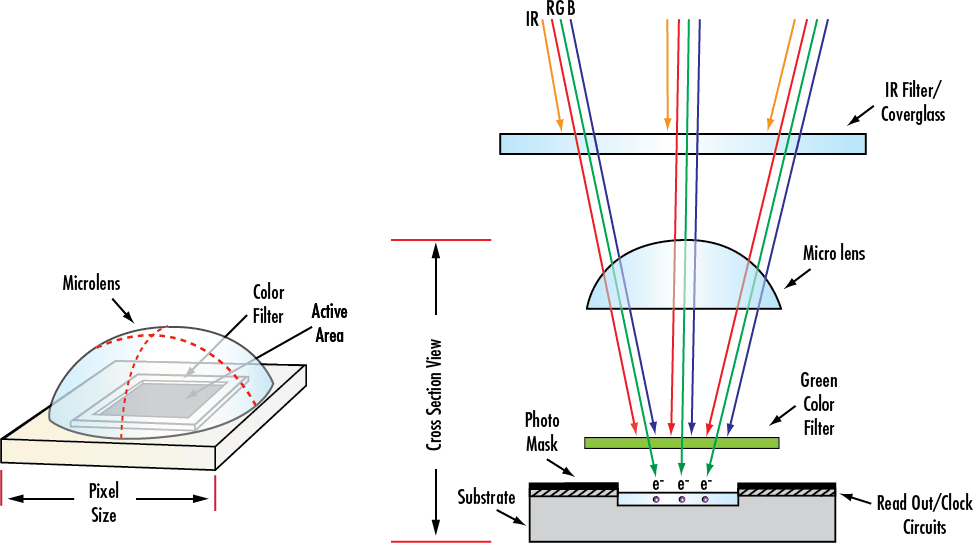
\includegraphics[width=.8\textwidth]{img/pixel.png}
\caption{Singolo elemento fotosensibile RGB con filtro NIR}
\label{fig:pixel}
\end{figure}

Telecamere CCD analogiche hanno pixel rettangolari (più grandi nella dimensione verticale). Questo è il risultato di un numero limitato di linee di scansione nelle norme di segnale (525 linee per NTSC, 625 linee per PAL) a causa di limitazioni di banda. Pixel asimmetrici producono risoluzione orizzontale superiore a quella verticale. Telecamere CCD analogicche (con lo stesso standard del segnale) di solito hanno la stessa risoluzione verticale. Per questo motivo, lo standard industriale di imaging è quello di specificare la risoluzione in termini di risoluzione orizzontale.

\subsubsection{Dimensione del sensore}

Le dimensioni dell'area attiva del sensore  è importante per determinare il campo visivo del Field of View (FOV). 
Dato un ingrandimento fisso (determinata dalla lente), sensori più grandi producono maggiori FOV. Ci sono diversi formati standard per sensori matriciali: 1/4'', 1/3'', 1/2'', 1/1.8'', 2/3'', 1'' e 1.2''. La nomenclatura di questi standard. risale ai tubi a vuoto vidicon utilizzati come imager per la trasmissione televisiva, per cui è importante notare che le dimensioni effettive dei sensori differiscono 

Un problema che si verifica spesso in applicazioni di imaging è la capacità di una lente di illuminare determinate dimensioni di sensore. Se il sensore è troppo grande per la lente, l'immagine risultante può apparire non illuminata uniformemente e l'illuminazione tende ad essere minore verso i bordi a causa di vignettatura (estinzione di raggi che attraversano i bordi esterni della lente di imaging). Questo è comunemente indicato come l'effetto tunnel, dal momento che i bordi del campo diventano scuri. Dimensioni del sensore più piccole non presentano questo fenomeno.

\begin{figure}[!ht]
\centering
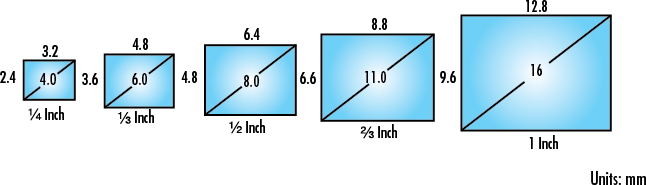
\includegraphics[width=.8\textwidth]{img/dimensione-sensore.png}
\caption{Dimensioni sensore}
\label{fig:dimensioni-sensore}
\end{figure}

\subsubsection{Frame rate e velocità dell'otturatore}
Il frame rate si riferisce al numero di immagini complete acquisite in un secondo.  Nelle applicazioni ad alta velocità, è utile scegliere un frame rate più veloce per acquisire più immagini dell'oggetto che si muove attraverso il FOV.

La velocità dell'otturatore corrisponde al tempo di esposizione del sensore. Il tempo di esposizione controlla la quantità di luce incidente. Il blooming (causato da eccessiva esposizione) può essere controllata diminuendo illuminazione, o aumentando la velocità dell'otturatore. Aumentare la velocità dell'otturatore può aiutare nella creazione di istantanee di un oggetto dinamico.

A differenza delle telecamere analogiche in cui, nella maggior parte dei casi, il frame rate è dettato dal display, le fotocamere digitali permettono un frame rate regolabile. Il frame rate massimo per un sistema dipende dalla velocità di lettura del sensore, la velocità di trasferimento dati dell'interfaccia compreso cablaggio, e il numero di pixel (quantità di dati trasferiti per frame). In alcuni casi, una telecamera può acquisire con un frame rate più elevato, riducendo la risoluzione o limitando l'area di interesse. Questo riduce la quantità di dati per frame, consentendo più fotogrammi da trasferire per una velocità di trasferimento fissa. Per una buona approssimazione, il tempo di esposizione è l'inverso della frequenza di quadro. Tuttavia, c'è un tempo minimo finito tra le esposizioni (dell'ordine di centinaia di microsecondi) a causa del processo di reset pixel e lettura, anche se molte fotocamere hanno la capacità quella di leggere la matrice mentre sta già subendo l'esposizione successiva (pipeline); 
Questo tempo minimo viene speso sull'elettronica della fotocamera.

Le telecamere CMOS hanno frame rate superiori, come il processo di lettura di ogni pixel può essere fatto più velocemente rispetto al trasferimento di carica nel registro a scorrimento di un sensore CCD.

\begin{figure}[!ht]
\centering
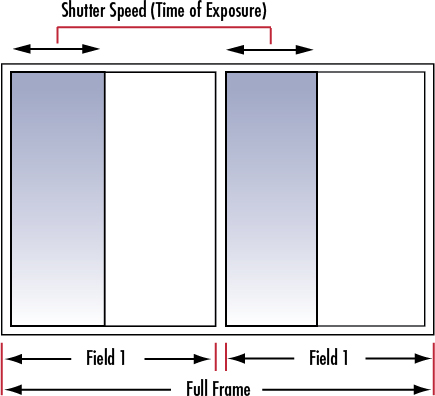
\includegraphics{img/shutter-speed.jpeg}
\caption{Velocità dell'otturatore}
\label{fig:shutter-speed}
\end{figure}

